%
% This file is part of Calicut University Question Paper Collection.
%
% Copyright (c) 2012-2015 Mohammed Sadik P. K. <sadiq (at) sadiqpk (d0t) org>.
% License: GNU GPLv3 or later
%
% Calicut University Question Paper Collection is free software: you can
% redistribute it and/or modify
% it under the terms of the GNU General Public License as published by
% the Free Software Foundation, either version 3 of the License, or
% (at your option) any later version.
% 
% Calicut University Question Paper Collection is distributed in the hope
% that it will be useful,
% but WITHOUT ANY WARRANTY; without even the implied warranty of
% MERCHANTABILITY or FITNESS FOR A PARTICULAR PURPOSE.  See the
% GNU General Public License for more details.
% 
% You should have received a copy of the GNU General Public License
% along with Calicut University Question Paper Collection.
% If not, see <http://www.gnu.org/licenses/>.
% 
%



\def \subj{ AI 09 604---ADVANCED CONTROL THEORY}

\mainhead{C 41262}{2}
\semsix{MAY 2013}
\sub{\subj}
\maxtime

\partA

\iitem Define Ackermann's formula.
\item Draw the structure of a full Order Observer.
\item Define State transition matrix. List out its properties.
\item Write the transfer function of a PI-controller.
\item Draw the graphical representation of stable, asymptotically stable, and unstable
      system in the sense of Liapunov.

\markA
\partB

\item What is Pole placement by state feedback and state oberserver.
\item Find the stability of the following system using Jury's test:

\hspace{2cm} F($z$)$ = 5z^2 - 2z + 2 = 0$.
\item Construct a state model for a system characterized by the differenct equations:

\hspace{2cm} $y (k+2) + 5y (k+1) +6y(k) = u(k)$.

\hspace{2cm} $y(0) = y(1) = 0; $ T$ = 1$sec.
\item What is a P-controller and what are its characteristics?
\item Show that the following quadratic form is positive definite:

\hspace{2cm} V($x$) $ = 10^2_1 + 4x_2^2 + x_3^2 + 2x_1x_2 - 2x_2x_3 - 4x_1x_3.$
\item Explain Liapunov stability analysis of LTI systems.

\markB

\newpage \again

\partC

\item  \iitem Investigate the controllability and observability of the following system:

\hspace{1cm}$\begin{bmatrix} \dot{x_1}\\\dot{x_2}\end{bmatrix} = \begin{bmatrix}
  -1 & 1\\
  0 & -1 \end{bmatrix} \begin{bmatrix}
  x_1\\ 
  x_2 \end{bmatrix} + \begin{bmatrix}
  0 \\ 1 \end{bmatrix}
u.$

\hspace{1.6cm}$y = \begin{bmatrix} 1 & 1 \end{bmatrix}
\begin{bmatrix}
  x_1\\ 
  x_2 \end{bmatrix}$
\item Consider the system with Transfer function G($s$)$ = 
  \dfrac{10}{s (s+1) (s+2)}.$ Design a state feedback
  controller so that the closed loop poles are placed at $-2, -1\pm j1.$
\ene
\item \iitem Obtain the state model of the following system G($s$) $
  = \dfrac{(s+3)}{(s+5)(s+2)^2}$.
\Or
\item Find the range of gains, K to make the system stable:

\begin{center}
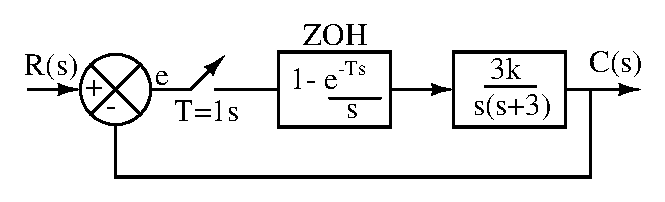
\includegraphics{src/s6/ai/09_604/fig1}
\end{center}
\ene

\item \iitem Explain the effects of proportional, integral, derivative and composite
  control modes on the response of a controlled process.
\Or
\item Write short notes on :
\iitem Ziegler Nichol's tuning.
\item Cohen and Coon tuning.
\ene \ene

\item \iitem Determine the stability of the equilibrium state of the following system using Liapunov
  method.

\hspace{2cm} $\dot{x}_1 = - x_1 - 2x_2$

\hspace{2cm} $\dot{x}_2 = x_1 - 4x_2$

\hspace{1cm} the Liapunov functions.
\Or
\item Explain robust Internal model control system in detail.
\ene

\markC
\ene

\newpage

\mainhead{C 26775}{2}
\semsix{MAY 2012}
\sub{\subj}
\maxtime

\partA

\iitem Draw the block diagram representation of the state equation.
\item Define a MIMO system.
\item List out different types of state space representations used.
\item Write the expressions of a PID controller transfer function.
\item Define `definiteness.' What are the different types of `definiteness'?

\markA
\partB

\item Briefly describe the configuration of an observer.
\item The input-output relation of a sampled data system is described by the equation

\hspace{1cm} $y(k+2) + 5y(k+1) + 6y(k) = x(k+1) - x(k).$ Determine its pulse transfer function.
\item Explain state transition matrix of discrete time system.
\item What is a PI controller and what are its effects on system performance?
\item Determine whether the following quadratic form is negative definite:

\hspace{1cm} V($x$) $ = -x_1^2 - 3x_2^2 - 11x_3^2 + 2x_1x_2 - 4x_2x_3 - 2x_1x_3.$
\item Briefly explain the Direct method of Liapunov stability analysis.

\markB

\newpage \again

\partC

\item \iitem Determine whether the following system is completely controllable and observable:

\hspace{1cm}$\begin{bmatrix} \dot{x_1}\\\dot{x_2}\end{bmatrix} = \begin{bmatrix}
  0 & 1\\
  -0.16 & -1 \end{bmatrix} \begin{bmatrix}
  x_1\\ 
  x_2 \end{bmatrix} + \begin{bmatrix}
  1 \\ -0.8 \end{bmatrix}
u,y = \begin{bmatrix} 1 & 0 \end{bmatrix}
\begin{bmatrix}
  x_1\\ 
  x_2 \end{bmatrix}$
\Or
\item Design a state feedback controller for the system $\dot{\text{X}} = \begin{bmatrix} 1 & -1\\
    1 & -2 \end{bmatrix} \text{X} + \begin{bmatrix} 1 \\ 2\end{bmatrix}u$ to place the poles
  at -1, -2.
\ene

\item \iitem Obtain the solutions of homogeneous and non-homogeneous state equations.
\Or
\item Consider a discrete time unity feedback control system (sampling period T = 1 sec.) whose
  open loop pulse transfer function is given by:

\hspace{1cm} G($z$) $ = \dfrac{\text{K} ( 0.3679z + 0.2642)}{(\text{Z} - 0.3679)(z -1)}$

  Determine the range of gains `K' for stability by use of Jury's stability test.
\ene

\item \iitem What are the different types of tuning techniques. Explain in detail.
\Or
\item Explain P, PI, PID controllers and obtain their circuitry realizations.
\ene

\item \iitem \iitem Briefly explain different types of definiteness with an example.
\item Consider the following system described by

  \hspace{1cm} $\mathring{x_1} = x_2$

  \hspace{1cm} $\mathring{x_2} = x_1 - x_2$

  Determine the stability of the system by Liapunove method.
\ene
\Or
\item Write short notes on:
\iitem Robust internal model control system.
\item Robust PID controlled systems.
\ene
\ene

\markC
\ene
